کد این بخش در \lr{solutions/Q8-nexus/} قرار دارد. کل پیکربندی به‌جای کلیک در رابط گرافیکی، از طریق \lr{REST API} نکسوس و در قالب اسکریپت انجام شده تا تکرارپذیر و قابل بازبینی باشد.

\subsectionaddtolist{الف) بالا آوردن نکسوس}

\begin{lstlisting}[language=Yaml]
services:
  nexus:
    image: sonatype/nexus3:3.79.1
    container_name: hw5-nexus
    environment:
      INSTALL4J_ADD_VM_PARAMS: "-Xms1g -Xmx2g -XX:MaxDirectMemorySize=2g"
    ports:
      - "8081:8081"   # UI + REST API + pypi/npm repository endpoints
      - "8082:8082"   # HTTP connector of the hosted docker registry
    volumes: [nexus-data:/nexus-data]
    ulimits: { nofile: { soft: 65536, hard: 65536 } }
    healthcheck:
      test: ["CMD", "sh", "-c", "curl -sf http://localhost:8081/service/rest/v1/status || exit 1"]
      interval: 15s
      retries: 40
      start_period: 60s
\end{lstlisting}

نکته: ایمیج \lr{sonatype/nexus3} تنها از نسخه‌ی \lr{3.78} به بعد \lr{arm64} منتشر می‌کند؛ تگ‌های قدیمی‌تر روی پردازنده‌های \lr{Apple Silicon} با شبیه‌سازی \lr{x86} اجرا می‌شوند که به‌شدت کند است.

\subsectionaddtolist{ب) مراحل انجام‌شده}

\begin{enumerate}
	\item {رمز اولیه}: نکسوس رمز تصادفی را در \lr{/nexus-data/admin.password} می‌گذارد؛ اسکریپت آن را می‌خواند و با یک درخواست \lr{PUT} تعویض می‌کند.
	\item {پذیرش \lr{EULA}}: نسخه‌های \lr{Community Edition} از \lr{3.78} به بعد تا وقتی توافق‌نامه پذیرفته نشود به {هر دانلود \lr{artifact}} پاسخ \lr{403} می‌دهند. نکته‌ی گمراه‌کننده این است که فهرست \lr{/simple/<pkg>/} با کد ۲۰۰ برمی‌گردد و فقط دریافت خود فایل رد می‌شود؛ خطا شبیه مشکل دسترسی به نظر می‌رسد ولی نیست.
	\item {\lr{Blob File}}: ساخت \lr{hw5-blob} از نوع \lr{File}.
	\item {مخازن \lr{Proxy}}: \lr{pypi-proxy} به \lr{https://pypi.org/} و \lr{npm-proxy} به \lr{https://registry.npmjs.org}، هر دو با \lr{storage} روی \lr{hw5-blob}.
	\item {مخزن \lr{Group}}: \lr{pypi-group} شامل \lr{pypi-proxy}.
	\item {\lr{realm} داکر}: فعال کردن \lr{DockerToken}.
	\item {مخزن داکر}: \lr{docker-hosted} با \lr{connector} روی پورت ۸۰۸۲ و \lr{writePolicy: ALLOW}.
\end{enumerate}

\begin{lstlisting}[language=bash]
create "pypi-proxy" /service/rest/v1/repositories/pypi/proxy '{
  "name": "pypi-proxy",
  "online": true,
  "storage": { "blobStoreName": "hw5-blob", "strictContentTypeValidation": true },
  "proxy":   { "remoteUrl": "https://pypi.org/", "contentMaxAge": 1440, "metadataMaxAge": 1440 },
  "negativeCache": { "enabled": true, "timeToLive": 1440 },
  "httpClient": { "blocked": false, "autoBlock": true }
}'
\end{lstlisting}

\begin{figure}[H]
\centering
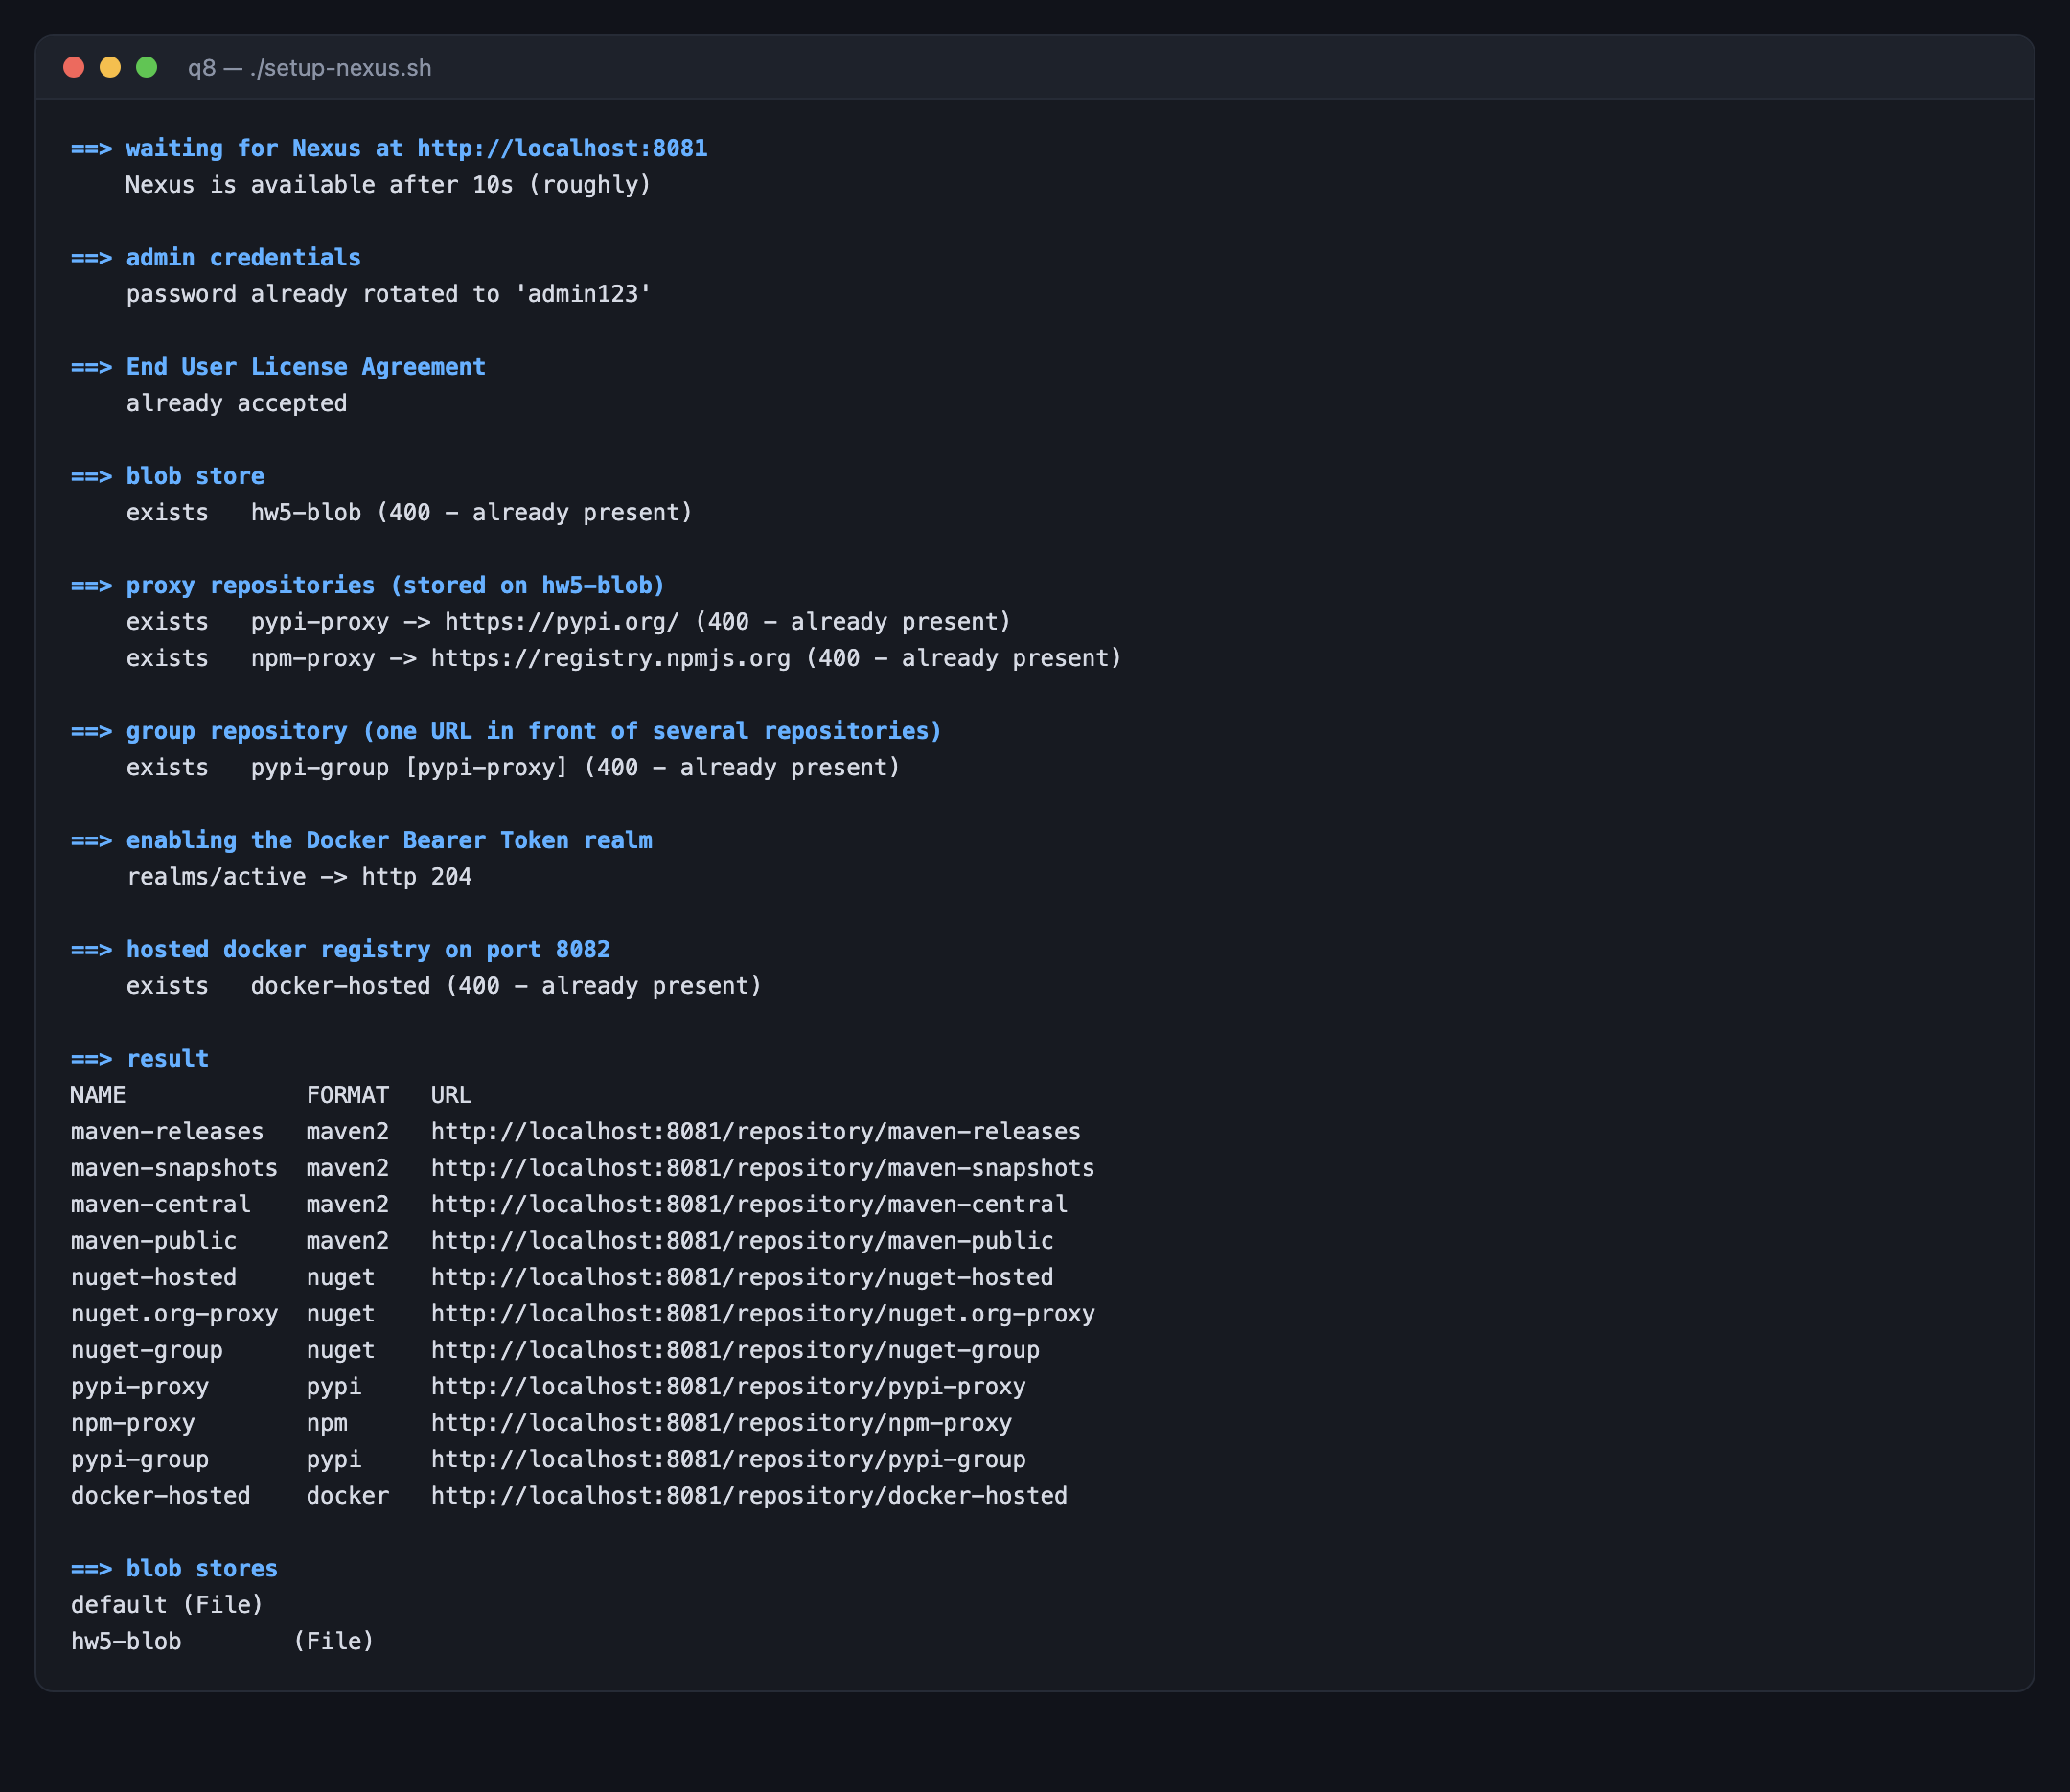
\includegraphics[width=0.95\textwidth]{figs/q8-setup.png}
\caption{خروجی \lr{setup-nexus.sh}؛ اسکریپت \lr{idempotent} است و اجرای دوباره‌اش چیزی را خراب نمی‌کند.}
\end{figure}

\subsectionaddtolist{ج) دریافت وابستگی‌ها از مخزن ساخته‌شده}

پروژه‌ی سؤال ۴ برای این کار استفاده شد؛ چون همان‌جا سازوکار \lr{MIRROR\_URL} پیاده شده بود، تنها کاری که لازم بود دادن نشانی نکسوس به‌عنوان \lr{index} است:

\begin{lstlisting}[language=bash]
docker build \
  --build-arg MIRROR_URL=http://host.docker.internal:8081/repository/pypi-proxy/simple \
  --build-arg MIRROR_TRUSTED_HOST=host.docker.internal:8081 \
  --target deps -t linkshrink:from-nexus ../Q4-dockerize
\end{lstlisting}

\subsectionaddtolist{د) پوش و پول ایمیج}

\begin{lstlisting}[language=bash]
docker login localhost:8082 -u admin
docker tag  alpine:3.20 localhost:8082/hw5/alpine:3.20
docker push localhost:8082/hw5/alpine:3.20
docker rmi  localhost:8082/hw5/alpine:3.20      # remove the local copy
docker pull localhost:8082/hw5/alpine:3.20      # pull it back from Nexus
\end{lstlisting}

\begin{figure}[H]
\centering
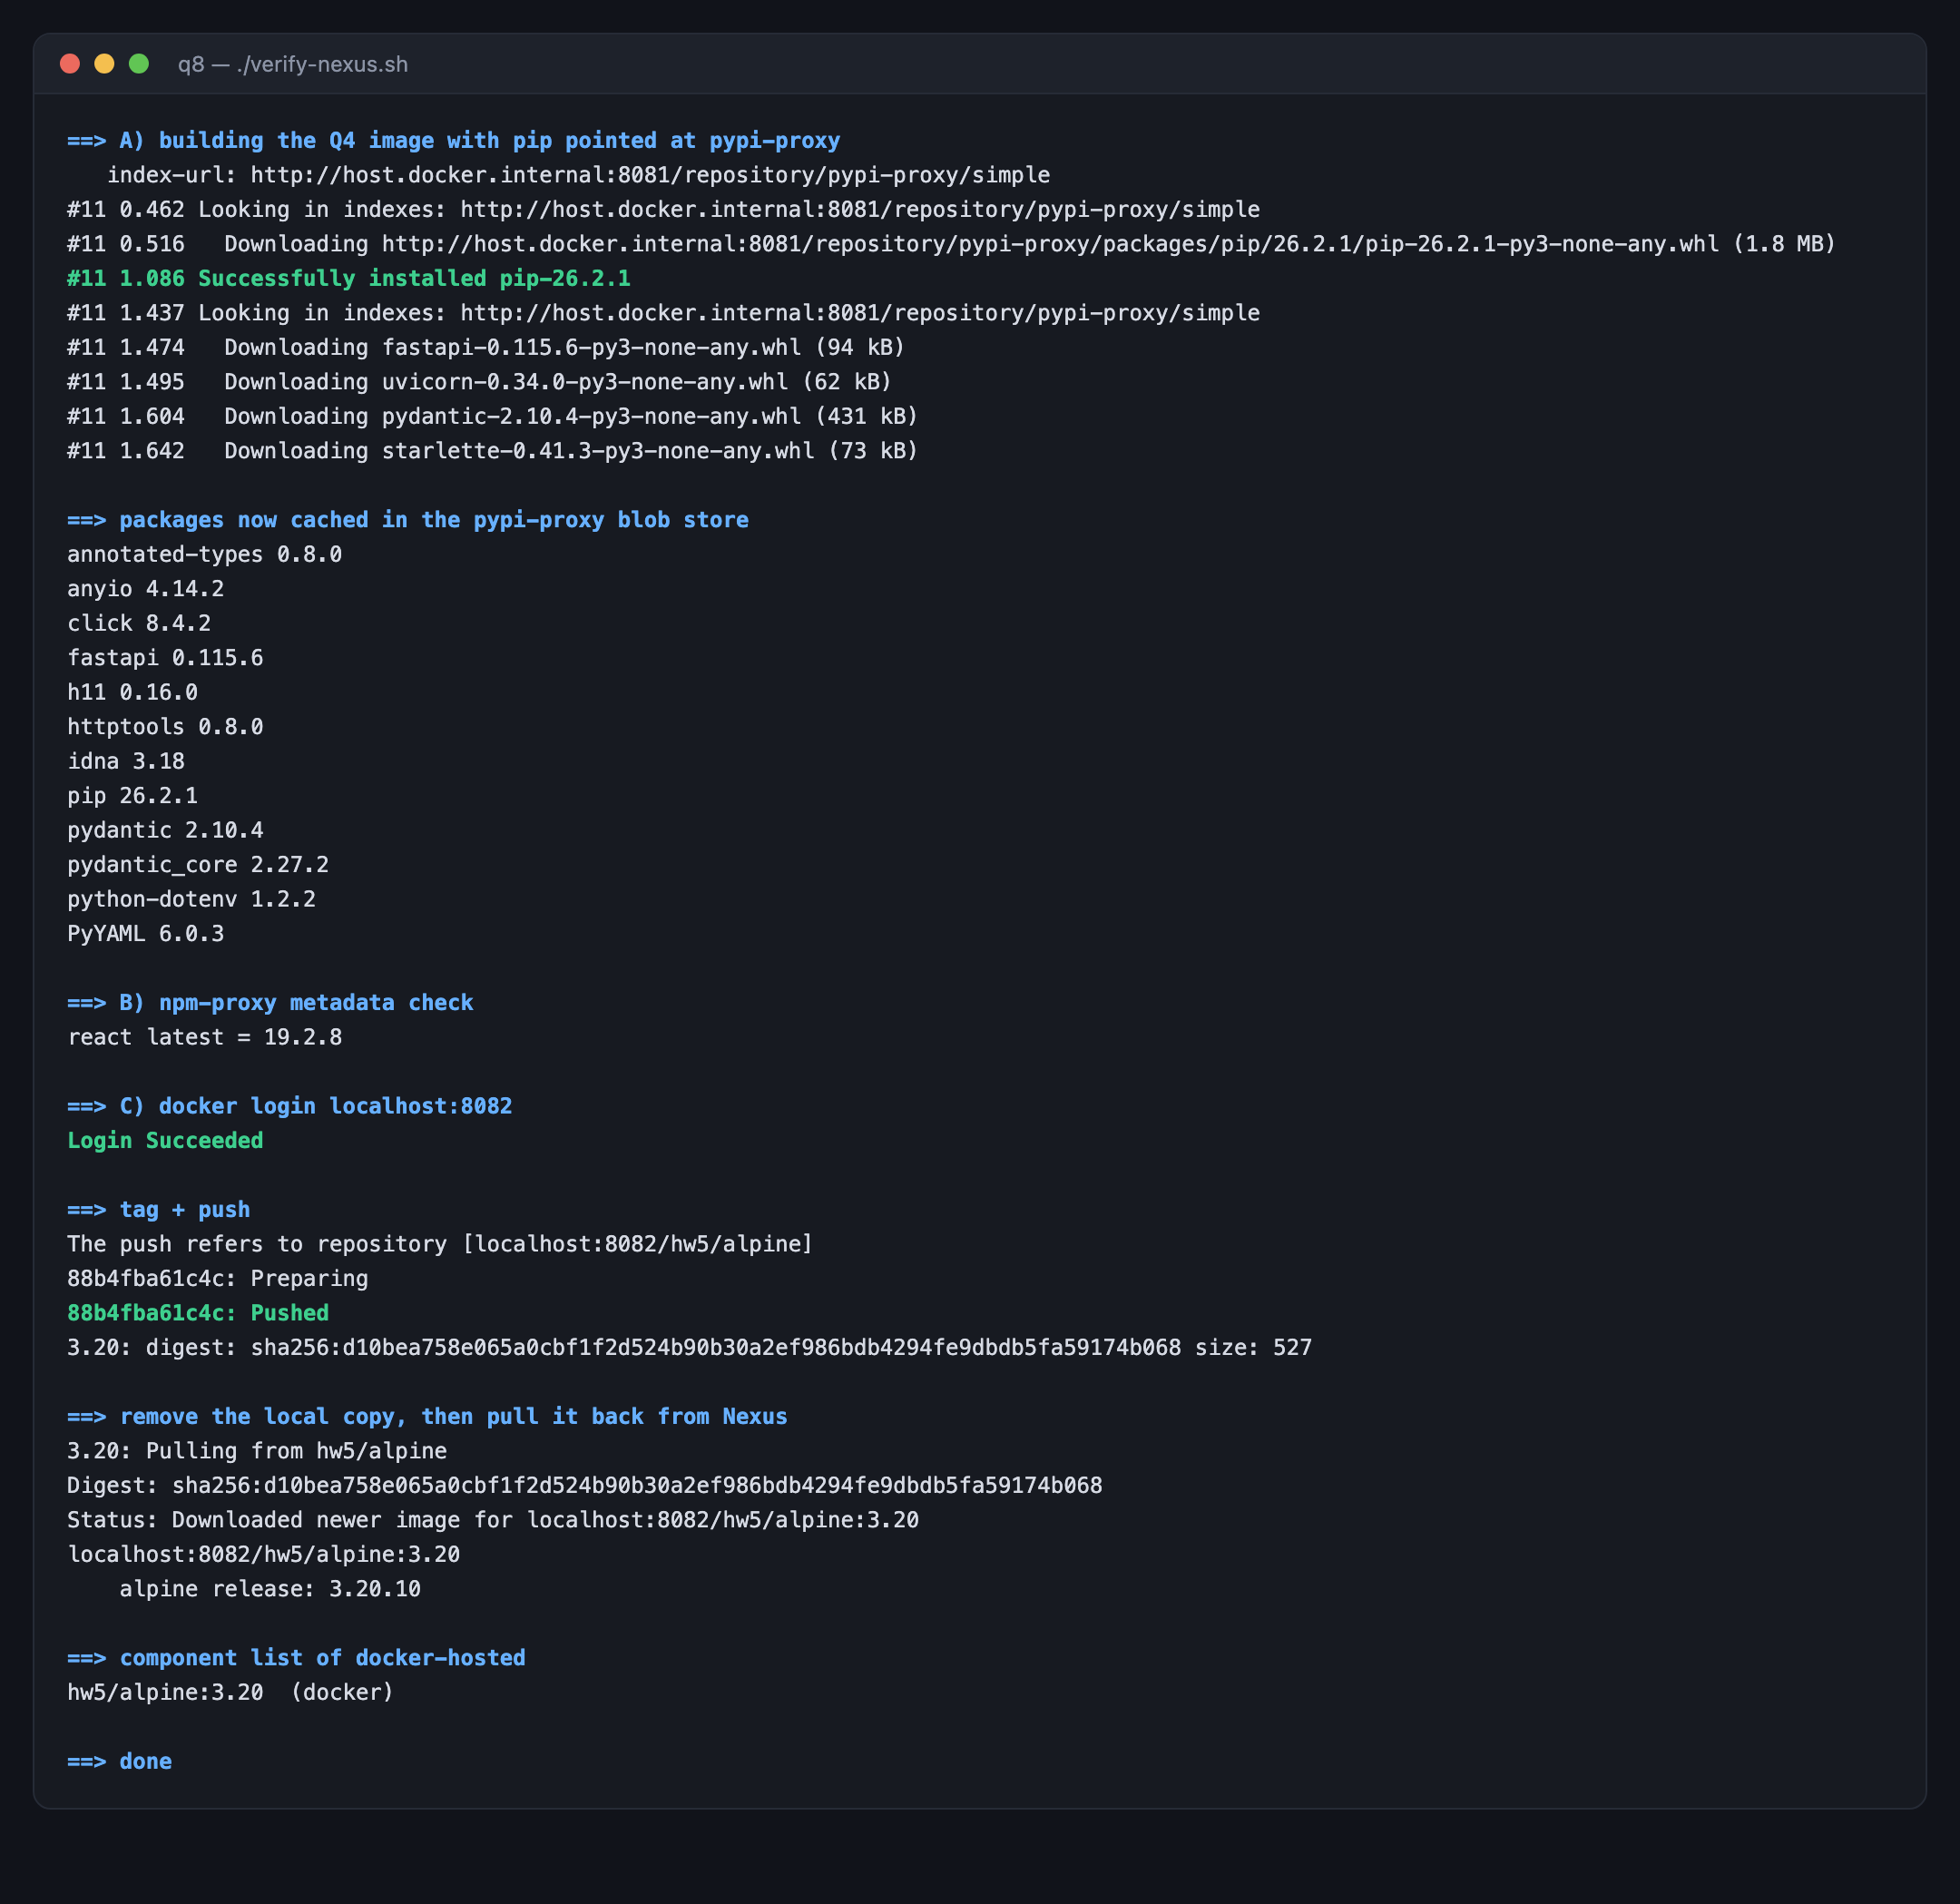
\includegraphics[width=0.95\textwidth]{figs/q8-verify.png}
\caption{خروجی \lr{verify-nexus.sh}: نصب وابستگی‌های پایتون از \lr{pypi-proxy} و کش شدن آن‌ها در \lr{blob store}، پاسخ \lr{npm-proxy}، و چرخه‌ی کامل \lr{login/push/pull} روی \lr{docker-hosted}.}
\end{figure}

یک نکته‌ی عملی که در مسیر به آن برخوردیم: با تنظیم پیش‌فرض (\lr{forceBasicAuth: false}) دستور \lr{docker login} با خطای \lr{unsupported protocol scheme "null"} شکست می‌خورد. علتش این است که جریان \lr{bearer token} نشانی \lr{token endpoint} را از قابلیت \lr{Base URL} نکسوس می‌سازد که در نصب تازه خالی است و از طریق \lr{REST API} عمومی هم قابل تنظیم نیست. راه‌حل، یا تنظیم \lr{Base URL} در رابط گرافیکی است یا فعال کردن \lr{forceBasicAuth} روی مخزن تا رجیستری با \lr{HTTP Basic} احراز هویت کند؛ راه دوم انتخاب شد چون کاملا در اسکریپت قابل انجام است.

\subsectionaddtolist{ه) نقش‌های نکسوس در یک پایپلاین \lr{CI/CD}}

\begin{enumerate}
	\item {کش و میرور وابستگی‌ها}: مخازن \lr{proxy} باعث می‌شوند بیلد به در دسترس بودن \lr{pypi.org} یا \lr{npmjs.com} وابسته نباشد. علاوه بر سرعت و کاهش ترافیک، در محیط‌هایی که دسترسی به اینترنت محدود یا فیلتر است، عملا تنها راه ادامه‌ی کار همین است.
	\item {مخزن \lr{artifact}های خودی}: خروجی بیلد (\lr{jar}، \lr{wheel}، پکیج \lr{npm} داخلی) در مخازن \lr{hosted} منتشر می‌شود و سرویس‌های دیگر با شماره‌ی نسخه آن را مصرف می‌کنند.
	\item {رجیستری ایمیج}: همان نقشی که در این تمرین دیدیم؛ نقطه‌ی تحویل بین \lr{CI} و \lr{CD}.
	\item {تفکیک نسخه‌های ناپایدار از پایدار}: جدا کردن \lr{snapshot} و \lr{release} در دو مخزن و اجازه‌ی \lr{promote} از اولی به دومی، به‌جای بیلد دوباره.
	\item {کنترل دسترسی و ممیزی}: نقش و کاربر جداگانه برای \lr{CI} (فقط خواندن از \lr{proxy}ها و نوشتن در \lr{hosted})، به‌همراه لاگ اینکه چه کسی چه چیزی را چه زمانی منتشر کرده است.
	\item {تکرارپذیری و امنیت زنجیره‌ی تأمین}: چون \lr{artifact} کش‌شده در نکسوس می‌ماند، حتی اگر نسخه‌ای از مخزن عمومی حذف شود بیلدهای قدیمی همچنان قابل بازتولیدند. همچنین می‌توان با قواعد \lr{Content Selector} و \lr{Routing Rule} جلوی ورود بسته‌های خاص یا آسیب‌پذیر را گرفت.
	\item {مدیریت چرخه‌ی عمر}: سیاست‌های \lr{cleanup} برای حذف خودکار \lr{snapshot}های قدیمی و ایمیج‌های بدون استفاده تا فضای دیسک کنترل شود.
\end{enumerate}

\subsectionaddtolist{و) کاربرد مخزن نوع \lr{Group}}

مخزن \lr{Group} خودش چیزی ذخیره نمی‌کند؛ چند مخزن {هم‌فرمت} را زیر {یک نشانی واحد} جمع می‌کند و درخواست را به‌ترتیب تعریف‌شده بین اعضا جست‌وجو می‌کند و اولین پاسخ را برمی‌گرداند.

فایده‌ی اصلی‌اش این است که کلاینت فقط {یک} نشانی می‌شناسد. برای مثال به‌جای اینکه در \lr{pip.conf} هر توسعه‌دهنده هم نشانی مخزن داخلی و هم نشانی \lr{proxy} نوشته شود، یک \lr{pypi-group} تعریف می‌کنیم که شامل \lr{pypi-hosted} (بسته‌های خودمان) و \lr{pypi-proxy} (بسته‌های عمومی) است. نتیجه:

\begin{itemize}
	\item پیکربندی سمت کلاینت ساده و ثابت می‌ماند؛ افزودن یک مخزن جدید فقط یک تغییر سمت سرور است و هیچ توسعه‌دهنده‌ای لازم نیست تنظیماتش را عوض کند.
	\item ترتیب اعضا معنادار است: قرار دادن مخزن داخلی {قبل} از \lr{proxy} باعث می‌شود بسته‌ی هم‌نام داخلی برنده شود؛ این هم برای اولویت‌دهی به کد خودی مفید است و هم یک لایه‌ی دفاعی در برابر حمله‌ی \lr{dependency confusion} است.
	\item در \lr{Group}های داکر، همین ویژگی اجازه می‌دهد یک \lr{endpoint} واحد هم ایمیج‌های داخلی و هم ایمیج‌های \lr{Docker Hub} را سرو کند.
	\item محدودیت مهم: \lr{Group} فقط برای {خواندن} است؛ برای انتشار باید مستقیما روی مخزن \lr{hosted} پوش کرد.
\end{itemize}
